The performances of the A* based ESM is tested for two different test scenarios. In scenario 1 the system is tested against a Sampling-Based Model Predictive Control (SBMPC) (CITE DOCTDER JOURNAL).In this case net metering is assumed to maintain similarity with the oter case. In scenario 2 the ESM is tested against two simple base test cases using both price data used in the first scenario and price data collected from PG\&E. In this scenario it is assumed buying and selling energy has different rates.

\subsection{Comparison with SBMPC and net metering}
 Model predictive control (MPC) uses a predictive model to optimize a cost function while enforcing constraints on the system inputs and outputs and is widely applied in industrial process control \cite{qin1997overview}. Typically, industrial MPC is implemented for linear models, but the use of nonlinear models allows better performance over a wider operating range \cite{berber2012nonlinear}. SBMPC \cite{dunlap2011book}, \cite{reese2016graph} is an MPC method that uses a receding horizon along with the optimization algorithm, Sampling-Based Model Predictive Optimization (SBMPO), which samples the input of the predictive model to compute a  graph tree with nodes and branches. In (CITE DOCTDER JOURNAL) the researchers use SBMPO to manage the energy at the PCC of a microgrid similar to the one described in section \ref{sys}.
 Figure \ref{fig:EMS_7_7days} shows the response of the A* based EMS for 7 days considering an energy storage price of 12.3 cents/kWh. The price of the energy storage is calculated according to the specifications of Tesla Powerpack \cite{tesla_powerpack_2018}. In the figure the blue line represents the real time price of energy. The dotted black line represents the price of using energy store age and the orange line represents the SOC of the energy storage. It can be seen in the figure that the A* based ESM is taking advantage of the lowest price before a price peak and charging the energy storage in order to discharge the energy storage when there is a high enough price peak to justify the use of the energy storage. Compared to the results of the method described in (CITE DOCTDER JOURNAL) the A* based method shows a savings of 50\$ in a seven day period.
 
 \begin{figure}[!ht]
    \centering
    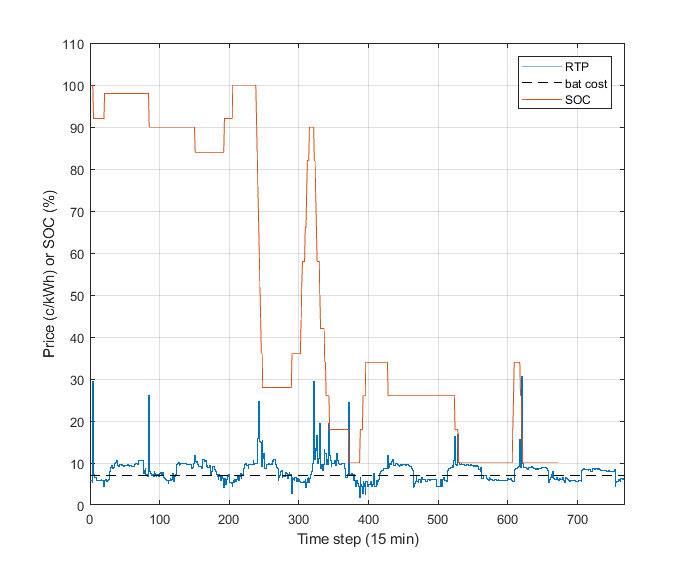
\includegraphics[width = \linewidth]{figs/Plot100_7.png}
    \caption{EMS response}
    \label{fig:EMS_7_7days}
\end{figure}


\subsection{Test result considering different buying and selling price}


